\documentclass[12pt,a4paper]{extarticle}
\usepackage[margin=1in]{geometry}
\usepackage[slantfont,boldfont]{xeCJK}
\usepackage{graphicx}
\usepackage{caption}
\usepackage{float}
\usepackage{pgfplots}
\usepackage{subcaption}

\graphicspath{{./images/}}
\pgfplotsset{compat=1.12}
\setCJKmainfont{cwTeXKai}

\title{Machine Learning 2017 Spring\\Homework 4 Report}
\author{學號:\texttt{B03902048}\\系級:資工三\\姓名:林義聖}
\date{}

\begin{document}
\maketitle

\begin{itemize}

  \item[1.1] Dataset 中前 10 個人的前 10 張照片的平均臉和 PCA 得到的前 9 個 eigenfaces。
  \par 答:平均臉呈現在 Figure \ref{fig:average-face},而 eigenfaces 在 Figure \ref{fig:top-9-eigenfaces}。

  \begin{figure}[ht]
    \begin{subfigure}[t]{0.5\textwidth}
      \centering
      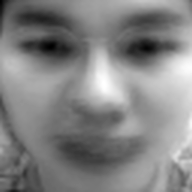
\includegraphics[width=0.8\linewidth]{average-face.png}
      \caption{The average face}
      \label{fig:average-face}
    \end{subfigure}
    \begin{subfigure}[t]{0.5\textwidth}
      \centering
      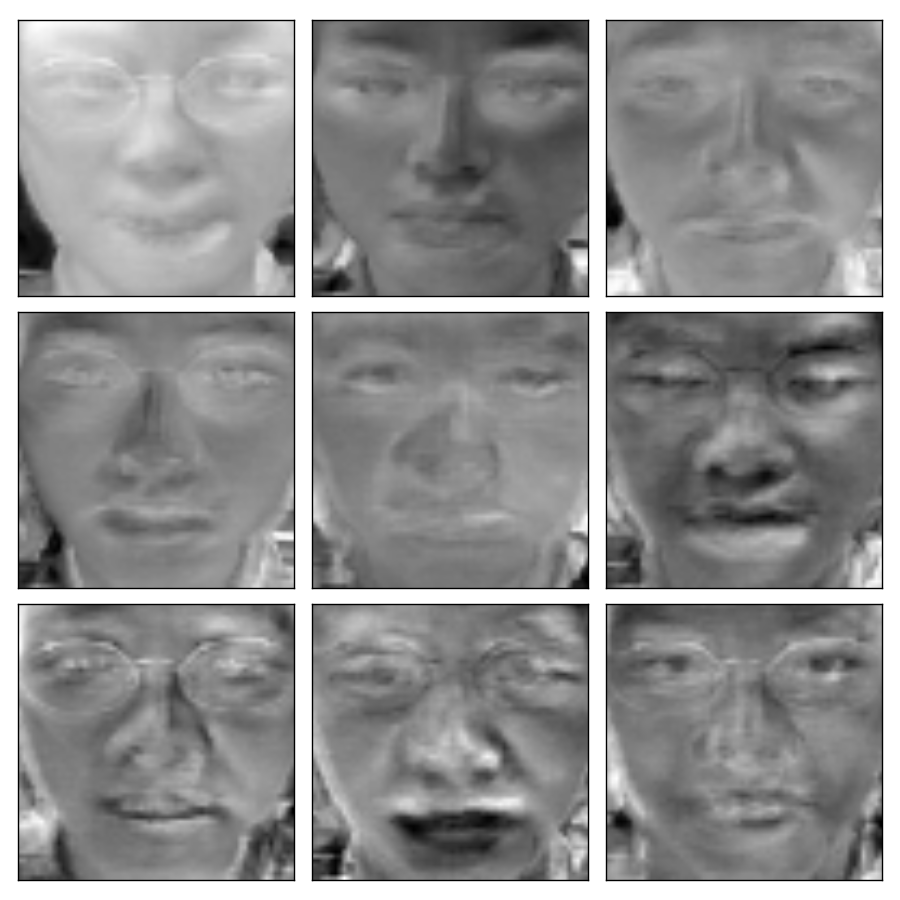
\includegraphics[width=0.8\linewidth]{eigen-faces-top-9.png}
      \caption{The top 9 eigenfaces}
      \label{fig:top-9-eigenfaces}
    \end{subfigure}
    \caption{}
  \end{figure}

  \item[1.2] Dataset 中前 10 個人的前 10 張照片的原始圖片和 reconstruct 圖(用前 5 個 eigenfaces)。
  \par 答:Figure \ref{fig:original-faces} 是原始圖片,而 Figure \ref{fig:recovered-faces} 是使用 eigenfaces 重建的圖片。

  \begin{figure}[ht]
    \begin{subfigure}[t]{0.5\textwidth}
      \centering
      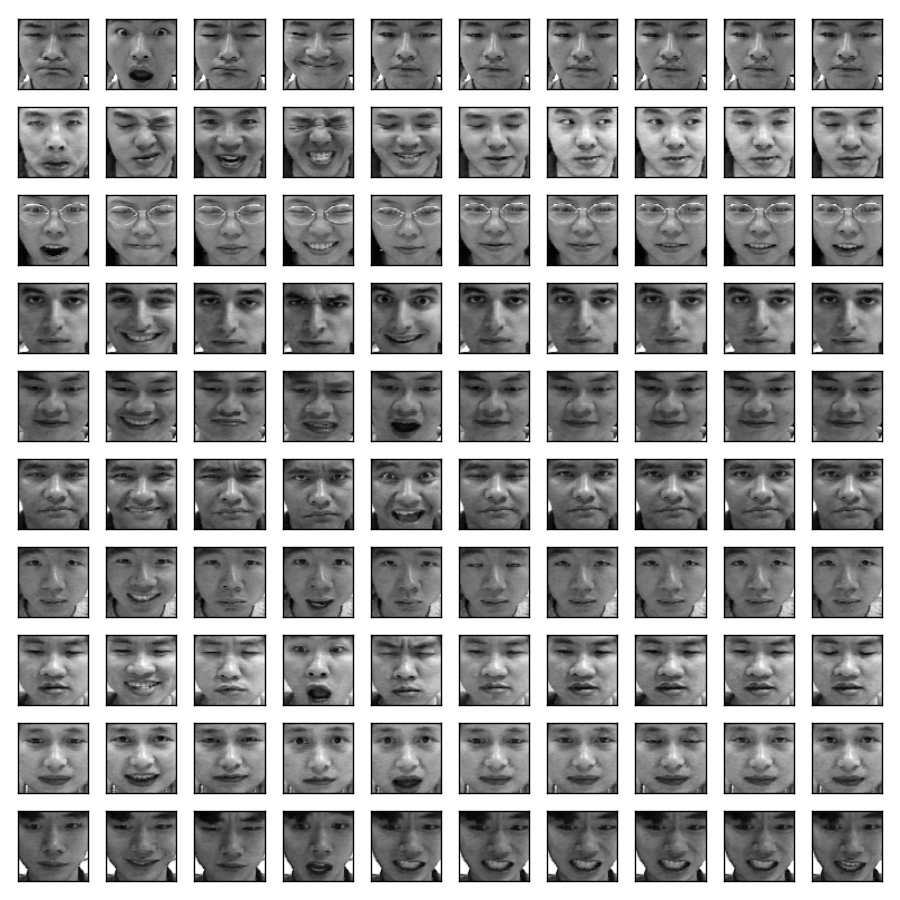
\includegraphics[width=\linewidth]{origin-faces-first-100.png}
      \caption{Original faces}
      \label{fig:original-faces}
    \end{subfigure}
    \begin{subfigure}[t]{0.5\textwidth}
      \centering
      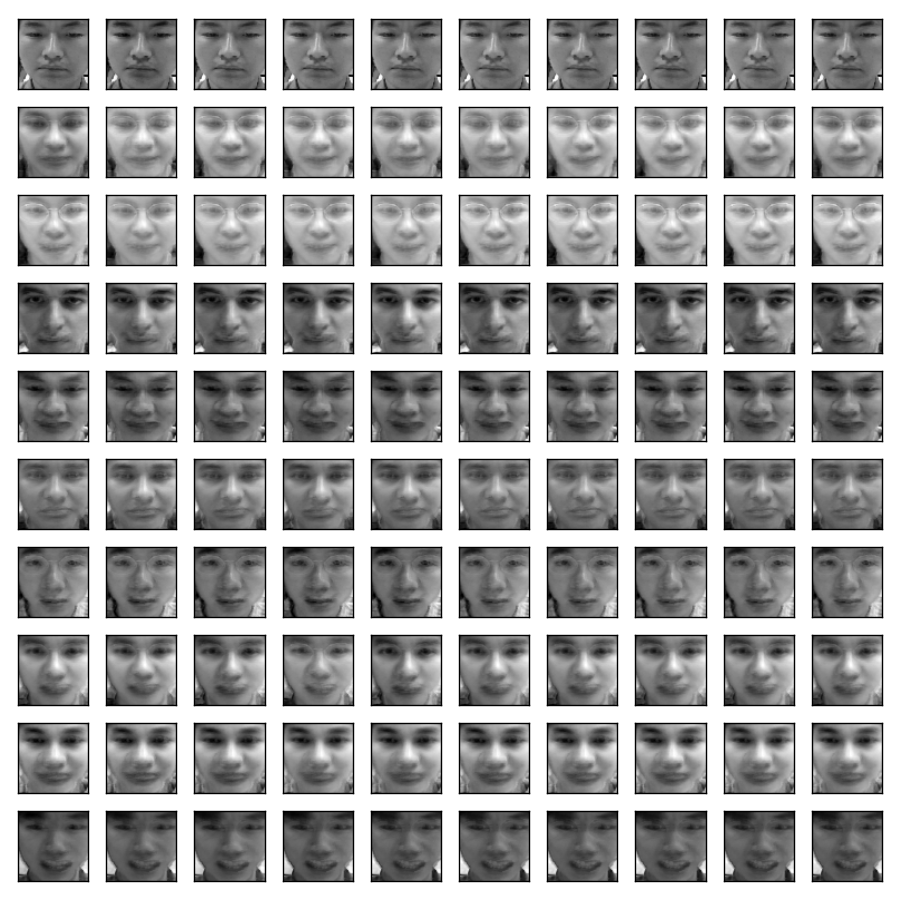
\includegraphics[width=\linewidth]{reconstruct-with-5-eigenfaces.png}
      \caption{Recovered faces}
      \label{fig:recovered-faces}
    \end{subfigure}
    \caption{100 faces reconstructed with top 5 eigenfaces}
    \label{fig:reconstruct-with-eigenfaces}
  \end{figure}

  \item[1.3] Dataset 中前 10 個人的前 10 張照片投影到 top $k$ eigenfaces 時就可以達到 < 1\% 的 reconstruction error?
  \par 答:當 $k = 59$ 時可以達到。

  % \begin{figure}[ht]
  %   \centering
  %   \begin{tikzpicture}
  %     \begin{axis}[
  %       ytick={0, 0.01, 0.02, 0.03, 0.04, 0.05, 0.06, 0.07, 0.08, 0.09, 0.1},
  %       xlabel = \# of eigenfaces,
  %       ymajorgrids]
  %     \addplot[color=blue] table [x=nb, y=rate, col sep=comma] {reconstruct-error.csv};
  %     \end{axis}
  %   \end{tikzpicture}
  %   \caption{Reconstruction error (RMSE)}
  %   \label{fig:eigenfaces-error-rate}
  % \end{figure}

  \item[2.1] 使用 word2vec toolkit 的各個參數的值與其意義。
  \par 答:我訓練 word2vec 模型時,使用的是 default 參數,並將 vector size 設為 64。
  \begin{itemize}
    \item word2phrase
    \par 有時原始的 data 中會有許多固定擺在一起的單字,如:地點、特殊名詞等,使用 word2phrase 可以將這樣的字組合起來視作一個單字。
    \item word2vec
    \begin{itemize}
      \item size:指定 vector size,將所有 word 以這個大小的 vector 表示
      \item window:指定 skip-gram 的最大 window 大小,亦即目標單字的左右,最多可能包含的字數
      \item sample:在訓練時,大於某個 frequency 的單字有機會被略過,即 down-sampled
      \item hs:指定是否使用 Hierarchical Softmax
      \item min\_count:指定是否忽略 frequency 小於這個數值的字
      \item alpha:即 learning rate 初始值
    \end{itemize}
  \end{itemize}

  \item[2.2] 將 word2vec 的結果投影到 2 維的圖。
  \par 答:我選擇頻率最高的 1000 個字,挑選過後剩下 381 個,呈現在 Figure \ref{fig:wordvec-es64-top1000}。

  \begin{figure}[ht]
    \centering
    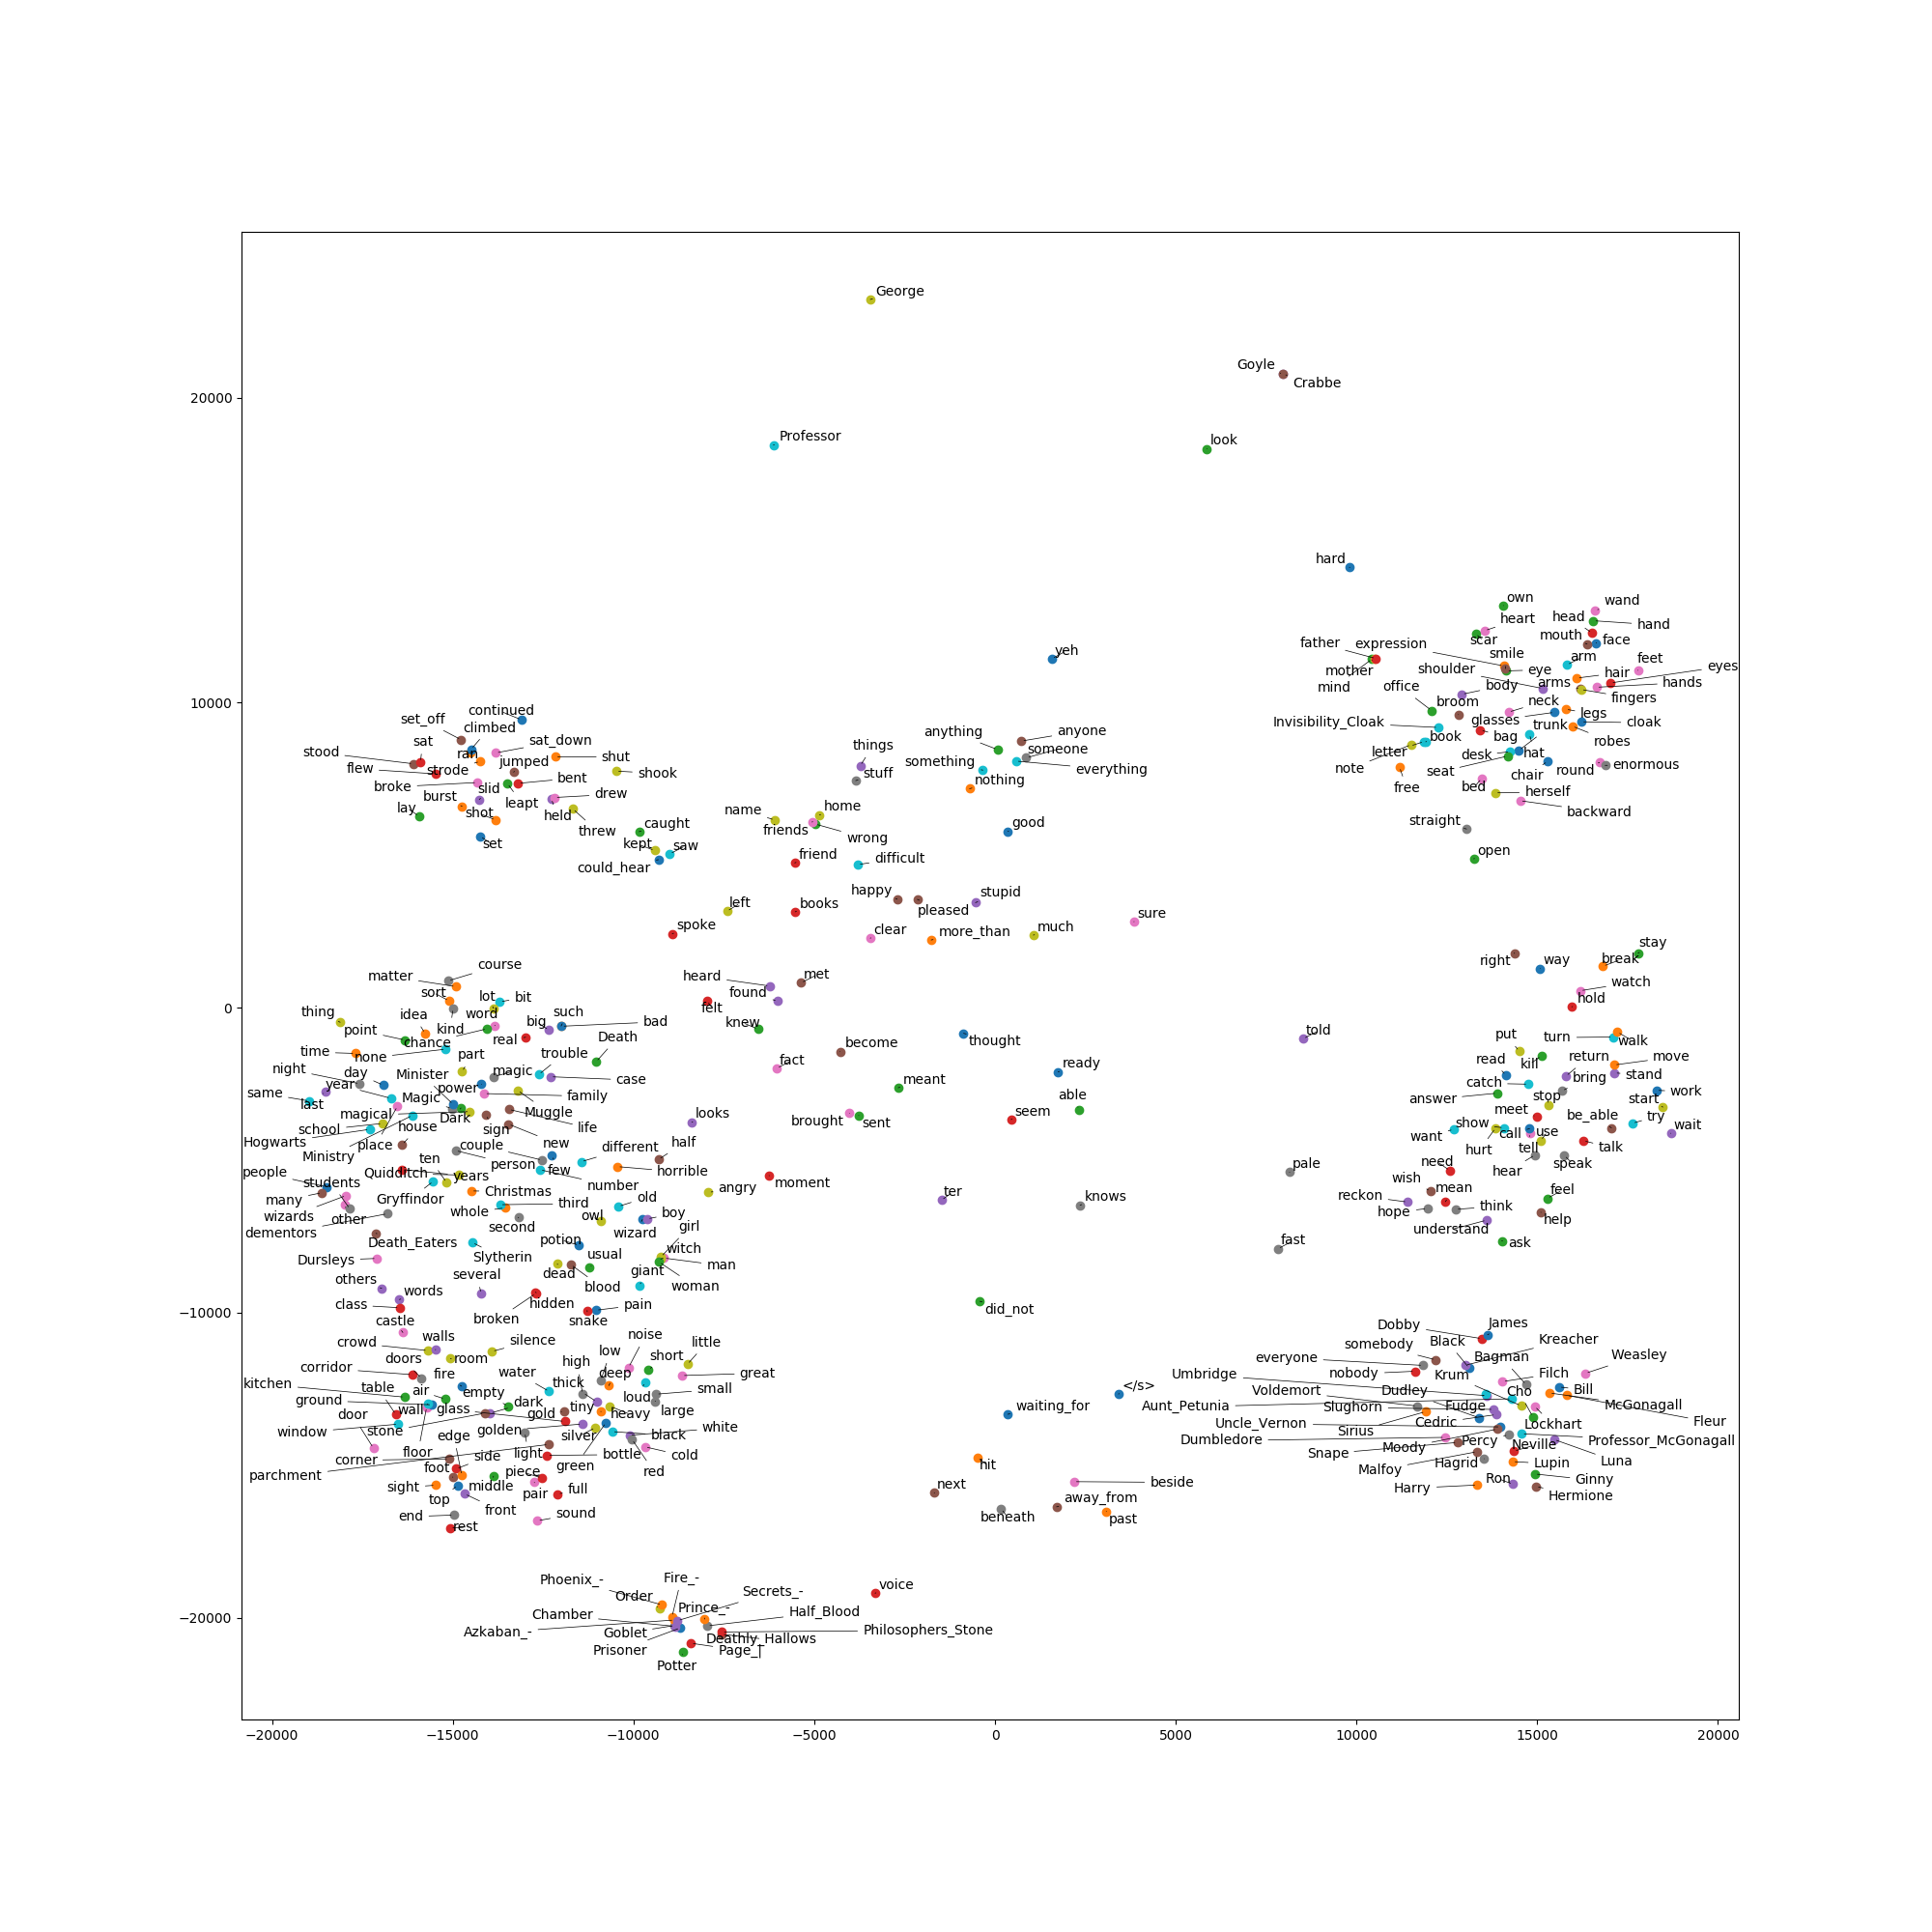
\includegraphics[width=0.8\linewidth]{images/wordvec-es64-top1000.png}
    \caption{The top 1000 frequent words}
    \label{fig:wordvec-es64-top1000}
  \end{figure}

  \item[2.3] 從上題視覺化的圖中觀察到了什麼?
  \par 答:從 Figure \ref{fig:wordvec-es64-top1000} 中,我觀察到「人名」聚集在圖片右下方,圖片右方中間則是一些「原型動詞」,右上方則比較特別,聚集了「身體部位」和「家具」。圖片最下方是「書名」,推測是因為訓練資料中每個頁面下方都會有書名,所以它們出現的頻率很高。圖片左下方是一堆「形容詞」,而鄰近它們的上方是一些「名詞」,圖片的左方偏上則是「過去式動詞」。

  \item[3.1] 請詳加解釋你估計原始維度的原理、合理性,這方法的通用性如何?
  \par 答:

  \item[3.2] 將你的方法做在 hand rotation sequence datatset 上得到什麼結果?合理嗎?請討論之。
  \par 答:

\end{itemize}

\end{document}
